%%
%% The Geneframe and Its Engine: typed, multi-kingdom Gene Expression
%% Programming on the GPU, with expression rewriting folded into the search.
%%
%% GECCO submission draft. House style (acmart sigconf), consistent with the
%% HFF papers. The body is venue-neutral; an EvoStar/EuroGP submission needs
%% only the LNCS preamble.
%%
\documentclass[sigconf,nonacm]{acmart}

\usepackage{amsmath}
\usepackage{booktabs}
\usepackage{listings}
\usepackage{tikz}
\usetikzlibrary{arrows.meta,positioning,shapes.misc,fit}

% A monospace style for regular expressions, genes and code.
\lstdefinestyle{mono}{basicstyle=\ttfamily\small, breaklines=true,
  columns=fullflexible, keepspaces=true}
\newcommand{\rx}[1]{\lstinline[style=mono]!#1!}
\newcommand{\ty}[1]{\textsf{#1}}

\begin{document}

\title{The Geneframe and Its Engine: Typed, Multi-Kingdom\\
Gene Expression Programming on the GPU}
\subtitle{One symbol table, three kingdoms, and expression rewriting folded into
the search}

\author{Andrew James Morgan}
\email{andrew@gamakon.ai}
\affiliation{%
  \institution{Gamakon Ltd.}
  \city{London}
  \country{United Kingdom}
}
\renewcommand{\shortauthors}{Morgan}

\begin{abstract}
Gene Expression Programming (GEP) encodes a program as a fixed-length linear
genome that decodes to an expression tree, and its genetic operators keep every
offspring valid without a repair step. That guarantee depends on closure: every
symbol must accept the output of every other, which classical GEP ensures by
admitting a single value type. We describe an architecture that extends GEP to
many value types and runs it on the GPU, split into two cooperating systems. The
\emph{geneframe} is one typed symbol table in which each symbol carries a
many-hot typed arity signature --- how many inputs of each type it consumes and
what type it produces --- and a \emph{kingdom} is a query over that table. A
\emph{total typed projection} decoder keeps every gene expressing under the
unchanged operators: a token whose output type does not match the type demanded
at its position is replaced by that type's fallback leaf. The evolutionary engine
holds the population resident on the device, decodes, varies and evaluates it in
compute kernels, and selects by hyperspherical fitness in tournaments that
reformulate the age-layered population structure as a cohort preference. The
rewriting system supplies in-search editors built on equality saturation:
simplification, constant snapping, and a new editor that finds subexpressions
shared across the genes of one chromosome, including sharing visible only after
rewriting. On this architecture we run three kingdoms. Untyped symbolic
regression is the single-type special case and decodes byte-for-byte as before.
Transcendental symbolic regression (TSR) gives the same operators a type that
records transcendental depth, so that a transcendental nested more than two deep
has no signature and does not express; on the 133 ground-truth SRBench problems
it recovers 74 laws in 90~s each on one development seed, and 79 once the
rewriting system generates candidates from the near misses. The third kingdom
evolves regular expressions over four value types on the same engine with no
change to variation or selection; a multi-typed detector for UK postcodes raises
held-out recall from 92.4\% to 97.5\% while rejecting every foreign-format
negative. The design is the contribution; the numbers are highlights, reported
with their conditions.
\end{abstract}

\maketitle

%% ===== SECTION 1 =====
\section{Introduction}
\label{sec:intro}

Gene Expression Programming~\cite{ferreira2001gep} is a form of genetic
programming~\cite{koza1992gp} in which the genotype is a fixed-length string of
symbols and the phenotype is an expression tree. Each \emph{gene} is a
K-expression: a \emph{head}, which may hold functions and terminals, followed by
a \emph{tail} of terminals only, read breadth-first into a tree. The tail is
sized from the maximum arity in the function set so that any arrangement of the
head decodes to a complete tree. A chromosome holds several genes whose trees are
combined by a fixed \emph{linker} (a sum, a product, or an average), so a
chromosome is a small ensemble of trees. The property that makes the
representation attractive is that mutation, transposition and recombination act
on the raw string and \emph{every} offspring still decodes to a valid program; no
repair is needed and no edit is wasted on an invalid individual.

That property depends on an assumption, closure: every symbol must accept, in
every argument slot, the output of every other symbol. Classical GEP enforces
closure by admitting one value type, so each symbol needs only an untyped operand
count and any output may fill any slot. This is adequate for symbolic regression,
where every operator consumes and produces a real number, although even there a
type can forbid shapes no law has, as Section~\ref{sec:geneframe} shows. It is
not adequate when the operators are typed. A counted repetition in a regular expression consumes a
pattern and an integer; a character class is assembled from characters and is a
different kind of value from a pattern. An operand count cannot express ``two
children, the first a pattern and the second an integer,'' and the raw operators,
which do not inspect types, will place an integer where a pattern is demanded.

This paper describes a representation, a decoder, and an engine that lift GEP to
many value types while keeping the raw operators and the every-gene-expresses
guarantee, and it describes the division of that engine into two cooperating
systems: \emph{phylu}, which evolves, and \emph{fuller}, which defines,
rewrites and evaluates expressions. The division is not an implementation detail.
It is what lets expression rewriting --- equality saturation over an e-graph ---
act as a mutation operator inside the search rather than as a post-processing
step, and it is what lets a genuinely multi-typed language run on the same
engine, beside two symbolic-regression kingdoms, without a line of
kingdom-specific selection code. The contributions are:

\begin{enumerate}
\item \textbf{The geneframe} (Section~\ref{sec:geneframe}): one typed symbol
table whose rows carry a many-hot typed arity signature, generalising Ferreira's
untyped operand count, with a \emph{kingdom} defined as a query over the table.
The total input arity equals the classical arity, so the tail-length rule
carries over unchanged.
\item \textbf{The total typed projection decoder} (Section~\ref{sec:decoder}): a
top-down decode carrying the type demanded at each position, in which a
mismatched token is replaced by the demanded type's fallback leaf and its subtree
becomes non-coding. Every gene expresses, the operators are untouched, and
heterogeneous types live in one gene. The count of substituted codons is kept as
a parity invariant between the host and device decoders and as the acceptance
gate on an edited gene. The first use of the typed table, the transcendental
depth ladder of the TSR kingdom, is narrower: a gene with no type derivation
does not express. Both decoders are in the engine and Section~\ref{sec:decoder}
states which kingdom uses which.
\item \textbf{A device-resident evolutionary loop} (Section~\ref{sec:engine}):
decode, variation and evaluation are compute kernels, and the population never
leaves the device during a generation. For the regular-expression kingdom the
match kernel runs a Thompson/Pike virtual
machine~\cite{thompson1968regex,cox2007regex,cox2009regexvm}, row-banded and
dispatched in two dimensions so that a full column fits the device's buffer
limits.
\item \textbf{Selection by hyperspherical fitness in cohort tournaments}
(Section~\ref{sec:selection}): fitness is the angular distance of a vector of
zero-seeking objectives from an ideal pole~\cite{morgan2026hff}; training and
validation error are both objectives; and the age-layered population
structure~\cite{hornby2006alps} is reformulated as a cohort label with a
same-cohort tournament preference, so young lines are protected without a
layered population.
\item \textbf{Rewriting folded into the search} (Section~\ref{sec:editors}):
the best individuals are decoded, edited by equality saturation~\cite{tate2009equality,%
willsey2021egg,egglog}, re-encoded into a valid typed gene, and returned to the
population for the tournament to judge. Three editors are built on this
template: simplification, constant snapping, and a shared-subexpression editor
that finds, across the genes of one chromosome, subtrees that are equal
\emph{after} rewriting, and executes them once.
\end{enumerate}

Section~\ref{sec:results} reports three highlights under their conditions ---
the SRBench ground-truth count, the postcode detector, and the measured economics
of shared subexpressions --- and Section~\ref{sec:limits} states what is not yet
done. We write for a reader who is comfortable with evolutionary computation but
may not have met GEP, e-graphs or many-objective fitness before, and we define
each on first use.

%% ===== SECTION 2 =====
\section{Related Work}
\label{sec:related}

Three families of prior work meet in this design. \emph{Typed genetic
programming} begins with Montana's strongly typed GP~\cite{montana1995stgp},
which enforces a type at every argument slot and makes the operators type-aware;
Ferreira's GEP~\cite{ferreira2001gep} takes the opposite route, keeping the
operators raw and enforcing closure by admitting one type. Our decoder lies
between them: the representation records the type relation, the operators stay
raw, and validity is recovered at decode time by projection
(Section~\ref{sec:decoder}). \emph{Equality saturation}~\cite{tate2009equality}
represents a space of equivalent expressions in one e-graph and extracts the
best member; egg~\cite{willsey2021egg} made it fast and egglog~\cite{egglog}
unified it with Datalog. We use it not as a compiler pass but as a mutation
operator, and we take from the database literature on DAG-shaped query
plans~\cite{neumann2009dag} the separation of whether sharing a subexpression is
\emph{legal} from whether it is \emph{worth it}. \emph{Many-objective selection}
without Pareto ranking is the subject of the hyperspherical fitness
work~\cite{morgan2026hff}; the age-layered population
structure~\cite{hornby2006alps} is the source of the protection of young
individuals that Section~\ref{sec:selection} reformulates.

Two application lines are relevant. Symbolic regression is evaluated on the
SRBench ground-truth track~\cite{lacava2021srbench}, on which AI
Feynman~\cite{udrescu2020aifeynman} is the reference physics-inspired method.
Learning regular expressions from examples by GP has been studied for text
extraction~\cite{bartoli2016regex}; our target is a data-quality assertion rule
scored by a confusion matrix on a label, with character-class masks as features.

%% ===== SECTION 3 =====
\section{Two Systems, One Loop}
\label{sec:architecture}

The engine is two Rust libraries with a one-way dependency: phylu depends on
fuller, never the reverse. Figure~\ref{fig:arch} shows the loop and
Table~\ref{tab:ownership} the division of responsibilities.

\begin{figure}[t]
\centering
\resizebox{\columnwidth}{!}{%
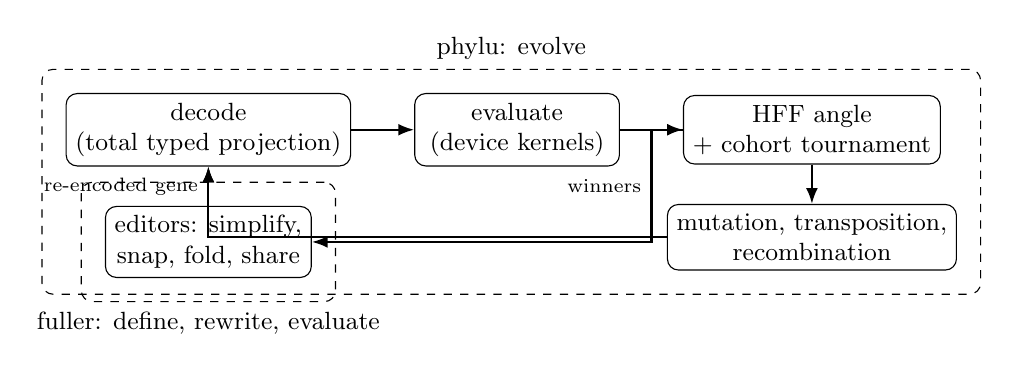
\begin{tikzpicture}[
  node distance=5mm and 8mm,
  box/.style={draw, rounded corners, align=center, minimum width=26mm,
              minimum height=8mm, font=\small},
  sys/.style={draw, dashed, rounded corners, inner sep=3mm},
  arr/.style={-{Latex[length=2mm]}, thick}
]
\node[box] (decode) {decode\\(total typed projection)};
\node[box, right=of decode] (eval) {evaluate\\(device kernels)};
\node[box, right=of eval] (hff) {HFF angle\\+ cohort tournament};
\node[box, below=of hff] (vary) {mutation, transposition,\\recombination};
\node[box, below=of decode] (edit) {editors: simplify,\\snap, fold, share};
\draw[arr] (decode) -- (eval);
\draw[arr] (eval) -- (hff);
\draw[arr] (hff) -- (vary);
\draw[arr] (vary) -| (decode);
\draw[arr] (hff.west) -- ++(-4mm,0) |- (edit.east) node[pos=0.25, left, font=\scriptsize]{winners};
\draw[arr] (edit) -- (decode) node[midway, left, font=\scriptsize]{re-encoded gene};
\node[sys, fit=(decode)(eval)(hff)(vary), label={[font=\small]above:phylu: evolve}] {};
\node[sys, fit=(edit), label={[font=\small]below:fuller: define, rewrite, evaluate}] {};
\end{tikzpicture}%
}
\caption{One generation. The population stays on the device through decode,
evaluation, selection and variation (phylu). Between generations the best
individuals of each island are passed to fuller, which rewrites them and returns a re-encoded
gene that replaces the island's worst individual, unevaluated, for the next
tournament to judge.}
\Description{A block diagram of the generation loop with the phylu and fuller
boundaries drawn as dashed boxes.}
\label{fig:arch}
\end{figure}

\begin{table}[t]
\caption{Division of responsibilities between the two systems.}
\label{tab:ownership}
\small
\begin{tabular}{@{}p{0.47\columnwidth}p{0.47\columnwidth}@{}}
\toprule
fuller (expressions) & phylu (evolution) \\
\midrule
the typed symbol table (geneframe) & GEP populations on the device \\
egglog rulesets and saturation & HFF selection, cohort tournaments \\
smallest-form and variant extraction & islands and random immigrants \\
constant snapping, physics priors & the in-search editor schedule \\
the device evaluator & telemetry, run cards, checkpoints \\
shared-subexpression detection & the two-pass shared evaluation \\
\bottomrule
\end{tabular}
\end{table}

\paragraph{Why two systems.} The rewriting layer has a different notion of
correctness from the evolutionary layer. A rewrite rule is sound or it is not;
an e-graph saturates or it grows without bound; an extracted expression either
is or is not a member of the input's equivalence class. None of this depends on fitness. The
evolutionary layer, by contrast, is indifferent to how a candidate was produced:
it decodes, scores, and selects. Keeping the two apart means that every editor
fuller offers --- a simplified form, a snapped constant, a shared subexpression
--- arrives in the population as an ordinary individual and is judged by the
same tournament as every other individual. We summarise the contract as \emph{fuller
proposes, the tournament disposes}. It also means that a new kingdom is added
by adding rows to fuller's table and kernels to phylu's evaluator, with
selection and variation untouched.

%% ===== SECTION 4 =====
\section{The Geneframe}
\label{sec:geneframe}

\subsection{A typed, many-hot symbol table}

The geneframe is one master symbol table. Each row is a symbol carrying a
kingdom label, an integer id (positive for a function, negative for a terminal),
a semantic identifier --- what the symbol computes, and the key an external
rewriter rewrites on --- a surface alias, and a \emph{typed arity signature}. The
signature is many-hot: rather than one integer it is a pair of maps from value
type to count,
\[
\ty{Arity} = \big(\ \mathrm{inputs}: \mathsf{Ty}\to\mathbb{N},\quad
\mathrm{outputs}: \mathsf{Ty}\to\mathbb{N}\ \big),
\]
so a symbol declares how many inputs of each type it consumes and what type it
produces. Classical GEP's arity is the special case in which inputs and outputs
are counted in one type. The total input arity $\sum_t \mathrm{inputs}(t)$ is
exactly Ferreira's integer arity, so the tail-length rule carries over
unchanged: a tail of length $h(a_{\max}-1)+1$ closes a head of length $h$.

A \emph{kingdom} is a query over the table: the symbols whose kingdom label
matches. The maximum total arity, used to size the tail, is derived per kingdom.
Adding a language is adding rows, not building a second engine. The value-type
enumeration is fixed and shared across kingdoms, so a new kingdom reuses the type
columns; a genuinely new value class is a new enumeration variant, added without
changing existing rows.

\subsection{Type safety at decode time}

Because each argument slot of each symbol has a declared type, a recombination
is type-correct exactly where a donor subtree's output type matches the
destination slot's input type. Rather than make every operator type-aware --- the
cost we avoid in Section~\ref{sec:decoder} --- type safety is obtained when the
genome is decoded: the decoder is a total function from any genome to a
well-typed tree, so any layout-respecting edit the raw operators produce still
yields a valid program. The representation records the type relation; the decoder
enforces it.

\subsection{The three kingdoms}

\paragraph{Symbolic regression: one float type.} The symbolic-regression
kingdom is the set of 26 real-domain operators --- arithmetic, powers, roots, the
reciprocal, the transcendentals, and their protected variants, which are
distinct symbols from the raw operators because they disagree on negative and
zero arguments. Every symbol consumes and produces the single float type
$\ty{F}$, the typed arity is a uniform float count, and the maximum total arity
is two. In this kingdom the type demand is always satisfied and the geneframe
reduces to the classical single-type table.

\paragraph{Transcendental symbolic regression: three depth types.} The TSR
kingdom holds the same 26 operators, but its type records \emph{transcendental
depth}: $\ty{F}$ is a plain float (a variable, a constant, or arithmetic over
plain floats), $\ty{T1}$ is the output of one transcendental applied to plain
floats, and $\ty{T2}$ is a transcendental applied to something already
$\ty{T1}$. Each operator is expanded into one row per accepted input
combination. Arithmetic is \emph{absorbing}: it accepts any mix of depths and
yields the highest it saw, six rows for a binary operator, so depth is carried
through $+$, $-$, $\times$ and $\div$. A transcendental (sine, cosine, tangent,
logarithm, exponential, root, absolute value, hyperbolic tangent, the inverse
trigonometric functions, and their protected forms) \emph{raises} depth by one
and has exactly two rows:
\begin{align*}
\ty{exp}&:\ \ty{F}\to\ty{T1}\\
\ty{exp}&:\ \ty{T1}\to\ty{T2}.
\end{align*}
There is no row accepting $\ty{T2}$, and no type above it. That missing row is
the whole design: a third nested transcendental is not penalised, it has no
signature and cannot be expressed. The ceiling was chosen by measurement. Over the 133 SRBench ground-truth models (128 parse), no law nests two
transcendentals directly; 78 lie at depth zero, 47 at depth one, 3 at depth two,
and none deeper. The three depth-two laws, such as
$\exp(-(\theta/\sqrt{2})^{2})$, reach that depth through arithmetic, which is
why arithmetic must absorb rather than reset. Every parsed law types under the
ladder, and 7 of 8 models the untyped engine had previously reported were
towers the ladder forbids.

\paragraph{Regular expressions: four value types.} The third kingdom evolves
regular expressions over \ty{Pattern} (the root type), \ty{CharClass},
\ty{Char} and \ty{Integer}. Representative rows, written as $\textit{inputs}\to
\textit{output}$:
\begin{align*}
\ty{concat}, \ty{alt}&:\ \ty{Pattern}\times\ty{Pattern}\to\ty{Pattern}\\
\ty{star}, \ty{plus}, \ty{opt}&:\ \ty{Pattern}\to\ty{Pattern}\\
\ty{rep\_n}&:\ \ty{Pattern}\times\ty{Integer}\to\ty{Pattern}\\
\ty{cc\_range}&:\ \ty{Char}\times\ty{Char}\to\ty{CharClass}\\
\ty{cc\_union}&:\ \ty{CharClass}\times\ty{CharClass}\to\ty{CharClass}\\
\ty{cc\_negate}&:\ \ty{CharClass}\to\ty{CharClass}\\
\ty{class\_of}&:\ \ty{CharClass}\to\ty{Pattern}.
\end{align*}
A \ty{CharClass} becomes a \ty{Pattern} only through the explicit \ty{class\_of}
operator, never implicitly, so the tree records exactly which type each node
holds. Terminals (the dot, anchors, the empty pattern and the built-in classes
\texttt{\textbackslash d}, \texttt{\textbackslash w}, \texttt{\textbackslash s})
carry an output type and no inputs. Every operator has
total arity at most two, the decoder's structural limit; a bounded interval is
composed from \ty{rep\_n} and a bounded repeat rather than carried as a
three-argument symbol.

%% ===== SECTION 5 =====
\section{The Total Typed Projection Decoder}
\label{sec:decoder}

\subsection{Three designs}

Three ways to admit types into GEP were weighed against three constraints: a
fixed-length device genome; raw, position-respecting operators (mutation,
transposition, recombination and the constant domain must not need per-operator
type logic); and every gene must express.

\begin{description}
\item[A --- type per position.] Ferreira's closure: a gene is mono-typed and
multiple types appear only across linked genes. The raw operators are kept, but a
single gene cannot represent $\ty{rep\_n}(\ty{Pattern},\ty{Integer})$. Too
restrictive.
\item[B --- type per slot.] Montana's strongly typed GP~\cite{montana1995stgp}:
heterogeneous genes, but every operator must become type-aware, or a repair step
is added, or validity drops below 100\%. This is the per-operator burden we must
not incur.
\item[C --- a total typed decoder.] Heterogeneous genes \emph{and} raw operators
unchanged. This is what we build.
\end{description}
The TSR kingdom was built first and lies between B and C: raw operators
unchanged and heterogeneous depth types in one gene, but a gene that does not
type is refused, so validity is below 100\%. That cost is what motivated C.

\subsection{The projection}

The decoder walks the tree top-down carrying the type \emph{demanded} at each
node. The root demands the kingdom's root type; a node's children inherit the
parent symbol's ordered per-slot input types. At a node whose token's output type
matches the demand, the token is decoded normally. At a node whose token's output
type does \emph{not} match, the decoder emits the demanded type's canonical
\emph{fallback leaf} and does not visit the token's would-be subtree, which
becomes non-coding. The decode is therefore total: every genome, however mutated
or recombined, projects to a well-typed tree. One zero-arity fallback is declared
per type; for the regular-expression kingdom they are the empty pattern for
\ty{Pattern}, the digit class for \ty{CharClass}, a fixed byte for \ty{Char},
and the count one --- a no-op repeat --- for \ty{Integer}.
Figure~\ref{fig:projection} shows the projection on a six-token head.

\begin{figure}[t]
\centering
\resizebox{\columnwidth}{!}{%
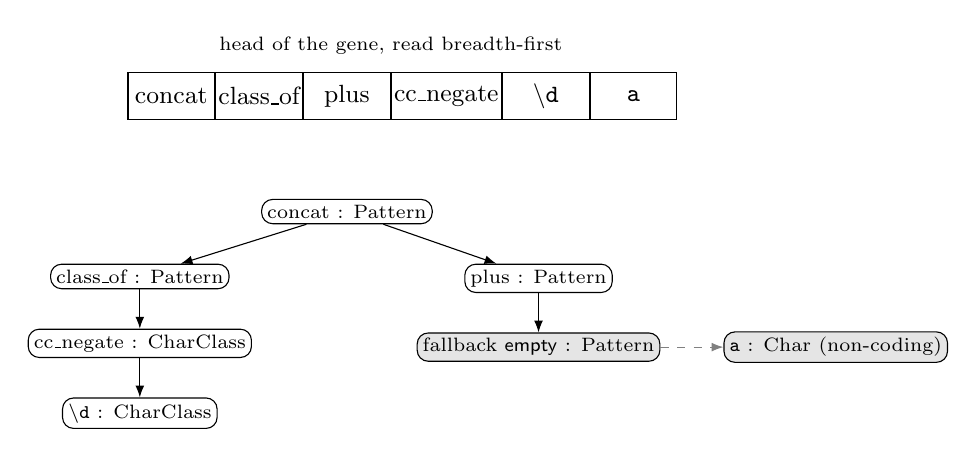
\begin{tikzpicture}[
  every node/.style={font=\small},
  tok/.style={draw, minimum width=11mm, minimum height=6mm, inner sep=1pt},
  lv/.style={draw, rounded corners, inner sep=2pt, font=\scriptsize},
  dead/.style={draw, rounded corners, inner sep=2pt, font=\scriptsize, fill=gray!20},
  arr/.style={-{Latex[length=1.5mm]}}
]
% the gene
\node[tok] (t0) {concat};
\node[tok, right=0mm of t0] (t1) {class\_of};
\node[tok, right=0mm of t1] (t2) {plus};
\node[tok, right=0mm of t2] (t3) {cc\_negate};
\node[tok, right=0mm of t3] (t4) {\texttt{\textbackslash d}};
\node[tok, right=0mm of t4] (t5) {\texttt{a}};
\node[above=1mm of t2.north east, font=\scriptsize] {head of the gene, read breadth-first};
% decoded tree
\node[lv, below=10mm of t2] (r) {concat : Pattern};
\node[lv, below left=5mm and 4mm of r] (a) {class\_of : Pattern};
\node[lv, below right=5mm and 4mm of r] (b) {plus : Pattern};
\node[lv, below=5mm of a] (c) {cc\_negate : CharClass};
\node[dead, below=5mm of b] (d) {fallback \ty{empty} : Pattern};
\node[lv, below=5mm of c] (e) {\texttt{\textbackslash d} : CharClass};
\node[dead, right=8mm of d] (f) {\texttt{a} : Char (non-coding)};
\draw[arr] (r) -- (a); \draw[arr] (r) -- (b);
\draw[arr] (a) -- (c); \draw[arr] (b) -- (d); \draw[arr] (c) -- (e);
\draw[arr, dashed, gray] (d) -- (f);
\end{tikzpicture}%
}
\caption{Total typed projection. \ty{plus} demands a \ty{Pattern} for its
child, but the token in that position, \texttt{a}, outputs a \ty{Char}; the
decoder emits the \ty{Pattern} fallback (the empty pattern) and the \texttt{a}
subtree is non-coding. The gene expresses as
\texttt{[\textasciicircum\textbackslash d](?:)+}, a valid program, with one
masked codon; no operator inspected a type.}
\Description{A six-token gene head above the typed tree it decodes to, with one
position replaced by a fallback leaf and its subtree greyed out as non-coding.}
\label{fig:projection}
\end{figure}

Two consequences follow. First, initialisation is demand-aware: head and tail
positions are drawn from symbols whose output type matches the top-down demand,
and \ty{Char} positions draw their literal from the gene's random-constant
domain, so most codons are productive from birth. Mutation, transposition,
recombination and the constant-domain operators are then left unchanged; the
projection absorbs whatever an edit moves out of type. Second, the projection
can \emph{neutralise} an edit by turning a mismatched subtree non-coding. The
decoder therefore counts the fallback substitutions per gene --- the
\emph{masked-codon} count --- and this count does two jobs. It is the invariant
of the host--device decode parity check: the CPU reference and the device
kernel must agree on which codons were masked, or the two decoders have
diverged. And it is the acceptance gate when an edited gene is re-inserted
(Section~\ref{sec:editors}): a re-encoded gene is accepted only if its masked
count is zero, which certifies that the re-inserted gene is a valid multi-typed
gene expressing with no fallback.

\subsection{Two decoders: refusal and projection}

The TSR kingdom was the first use of the typed table and it types the other way
round. After the Karva walk has laid out the node array, the device decoder
derives a type for every node bottom-up, in reverse index order, since a child's
index is always greater than its parent's: a terminal is $\ty{F}$, an absorbing
operator takes the maximum of its children, a raiser adds one. A raiser over
$\ty{T2}$ has no row, and a gene with no derivation does not express: its
program has length zero and it is counted as \emph{refused}, separately from the
count of genes that exceed the node limit. Initialisation and variation draw
under a per-position depth budget --- the ceiling at the root, a child's budget
being its parent's less the parent's cost --- which reduces refusals but is not
the guarantee; the decoder is. The budget and the bottom-up derivation compute
the same predicate, the largest transcendental count on any root-to-leaf path,
and that agreement is a test. A refused gene is not a dead individual: a
chromosome of three genes scores on its other two, and the refused gene is
carried unscored and keeps varying. That is the honest limit of
``unrepresentable'' at the chromosome level, and it is why the final
population of a TSR run still holds genes past the ceiling.

Design C, the projection above, generalises the ladder to
heterogeneous types and makes every gene express; it is the decoder of the
regular-expression kingdom, and the TSR ladder has not yet been re-expressed
through it. Design C is a strict superset of the classical decode: in a
single-type kingdom the demand is always satisfied, the fallback is never used,
the masked count is identically zero, and the decode reduces to the classical
path. The untyped symbolic-regression kingdom, with both typings off, is held
byte-identical against a golden population pinned before either typing existed
and against the CPU reference decode; the TSR decode is held to host--device
parity on fixtures and to lockstep with the symbol table's rows. The typing is
therefore an extension of the existing engine and not a perturbation of it.

%% ===== SECTION 6 =====
\section{The Engine on the Device}
\label{sec:engine}

A population is a flat buffer of 32-bit tokens and 32-bit constants held
resident on the device across generations. Decode, variation and evaluation are
compute kernels in WGSL, three command submissions per generation (variation,
decode, and the fitness chain), and the population never leaves the device in
the hot loop. Each device kernel has a
bit-exact host reference, and the regular-expression kernels are additionally
cross-checked against an independent engine (Rust's \texttt{regex} library) as an
oracle.

\paragraph{Symbolic regression.} The evaluator is fuller's: a gene decodes to a
flat node array in level order, each node holding an opcode and local child
indices, and one kernel evaluates every node of every gene over every row of the
resident data set. Objective columns ($1\!-\!R^2$, mean squared error, mean
absolute deviation; each on training and on validation rows) are reduced on the
device.

\paragraph{Regular expressions.} A gene decodes to a node array; a compile kernel
lowers it to a Thompson/Pike virtual-machine
program~\cite{thompson1968regex,cox2007regex,cox2009regexvm} with the
instructions \texttt{Char}, \texttt{AnyByte}, \texttt{Class}, \texttt{Assert},
\texttt{Split}, \texttt{Jmp} and \texttt{Match}; a match kernel runs the program
over every labelled value as a program-counter-bitmask NFA, $O(n\cdot m)$ in
program and input size, with no backtracking. The match is the one kernel whose
work is cubic --- population $\times$ genes $\times$ rows --- and a single flat
dispatch over that product overran the device buffer limit on a realistic column;
the match and the score are therefore \emph{banded} over row chunks and
dispatched in two dimensions. Malformed trees that recombination can produce (an
out-of-range child index, a self-reference, a disconnected node) are refused by
the same checks in the same order on host and device; on the device such a gene
compiles to an empty program, which matches nothing.

\paragraph{Throughput.} Table~\ref{tab:throughput} gives representative
generation times on an Apple Silicon laptop through the Metal backend of wgpu.
The move from the original Python engine to the device engine is a factor of
about 34 at a population of 800; from there the generation time grows
sub-linearly in population, and the regular-expression kingdom, whose match is
the heavier kernel, still sustains a quarter of a million individuals per second
at a population of 2{,}600.

\begin{table}[t]
\caption{Generation time and throughput, one seed, Apple Silicon via wgpu/Metal.
Untyped symbolic-regression figures are on Feynman problems at the engine's
default data split (up to 4{,}000 training rows), taken on the 21 September
2026 build, before the device-resident generation described above made the
engine faster (Strogatz shear flow fell from 58 to 12.5~ms per generation across
that rebuild with identical trajectories), so they are conservative. The TSR
row is the Strogatz shear-flow run of the SRBench study (240 training rows).
Regular-expression figures are on the postcode task of
Section~\ref{sec:results-regex}, the same two runs as Table~\ref{tab:regex}.
Individuals per second are derived from the logged generation counts and run
times, not measured separately.}
\label{tab:throughput}
\small
\begin{tabular}{@{}lrrr@{}}
\toprule
Configuration & Pop. & ms/gen. & Indiv./s \\
\midrule
Python engine (reference) & 800 & 1{,}200 & 670 \\
Device, SR untyped & 800 & 35 & 23{,}000 \\
Device, SR untyped & 2{,}000 & 46 & 43{,}000 \\
Device, SR untyped & 20{,}000 & 176 & 114{,}000 \\
Device, SR untyped & 40{,}000 & 296 & 135{,}000 \\
Device, TSR & 2{,}000 & 15.5 & 129{,}500 \\
Device, regex, single-type & 2{,}600 & 21 & 125{,}000 \\
Device, regex, multi-typed & 2{,}600 & 10 & 253{,}000 \\
\bottomrule
\end{tabular}
\end{table}

%% ===== SECTION 7 =====
\section{Selection: Hyperspherical Fitness in Cohort Tournaments}
\label{sec:selection}

\subsection{Hyperspherical fitness}

Selection is by hyperspherical fitness (HFF)~\cite{morgan2026hff}. Each
individual is scored on a vector of $m$ objectives $\mathbf{x}$, each scaled
into $[0,1]$ with $0$ best. The \emph{TrueNorth} pole is the ideal point at which
every objective vanishes; fitness is the angular distance from that pole:
\[
\theta \;=\; \arccos\!\Big(1 - \min\big(\tfrac{1}{m}\textstyle\sum_i x_i^2,\ 1\big)\Big),
\]
where the cosine is the normalised energy of the objective vector, so
$\theta=0$ exactly at the pole and larger the farther the individual lies from
it (Figure~\ref{fig:hff}). Because the objectives enter one angle, many
heterogeneous objectives stay comparable without hand-tuned weights, and the
angle is computed on the device for the whole population each generation.
Selection is then tournament selection on the scalar $\theta$, lower preferred.

\begin{figure}[t]
\centering
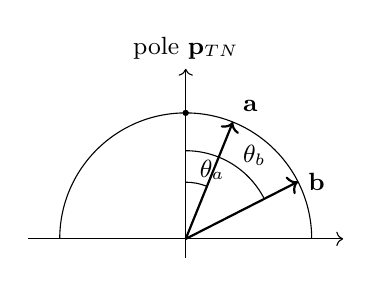
\begin{tikzpicture}[scale=1.6, every node/.style={font=\small}]
  \draw[->] (-1.25,0) -- (1.25,0);
  \draw[->] (0,-0.15) -- (0,1.35) node[above] {pole $\mathbf{p}_{TN}$};
  \draw (1,0) arc (0:180:1);
  \fill (0,1) circle (0.025);
  \coordinate (A) at ({sin(22)},{cos(22)});
  \coordinate (B) at ({sin(63)},{cos(63)});
  \draw[->, thick] (0,0) -- (A) node[above right] {$\mathbf{a}$};
  \draw[->, thick] (0,0) -- (B) node[right] {$\mathbf{b}$};
  \draw (0,0.45) arc (90:68:0.45) node[midway, above right, inner sep=1pt] {$\theta_a$};
  \draw (0,0.7) arc (90:27:0.7) node[pos=0.6, above right, inner sep=1pt] {$\theta_b$};
\end{tikzpicture}
\caption{Hyperspherical fitness. Each individual's objective vector is placed on
the unit sphere; fitness is its angular distance from the pole, where every
objective is zero. Individual $\mathbf{a}$ (smaller $\theta$) is preferred over
$\mathbf{b}$ in a tournament. Lower is better.}
\Description{A unit semicircle with the pole at the top and two objective
vectors at different angles from it.}
\label{fig:hff}
\end{figure}

Three choices in how the objective vector is assembled matter here.

\paragraph{Many objectives, all zero-seeking.} Every objective is a rate or a
scaled error oriented so that $0$ is best and $1$ is worst; the pole is the
common ideal and no objective needs a separate target direction. For symbolic
regression the objectives are the $1\!-\!R^2$, MSE and MAD columns; for the
regular-expression kingdom they are confusion-matrix error rates.

\paragraph{Training and validation are both objectives.} Generalisation is built
into selection rather than applied afterwards. The vector carries the error
measured on the training rows \emph{and} the same error on a validation block
the search can see, so an individual that fits the training rows but not the
validation rows lies farther from the pole and is selected against. For the
regular-expression kingdom the default set is the confusion matrix on training
and again on validation --- eight columns: the false-negative rate (a good value
rejected) and the false-positive rate (a bad value accepted), each listed twice
per block so that each is weighted inside the angle. A third, held-out split is
never an objective and never gates the search; it is scored once, on the final
individual.

\paragraph{No parsimony objective.} A length objective is available but off by
default. On the small alphabet of the regular-expression kingdom a length
pressure collapses the search onto a few short, loose rules and destroys
diversity; for symbolic regression it is likewise not a default objective.
Compactness comes instead from the editors of Section~\ref{sec:editors}.

\subsection{Cohort tournaments: the age-layered structure reformulated}

The age-layered population structure (ALPS)~\cite{hornby2006alps} protects young
genetic material from being out-competed before it has had time to develop, by
keeping age-indexed sub-populations with restricted migration and a periodically
reseeded youngest layer. We want that protection without carrying separate
sub-populations across the device, so we reformulate it inside the tournament.
Every individual carries a \emph{cohort} label: the immigration interval on
which its founding line arrived, inherited by every descendant. (Islands run in
pairs. Every fixed number of generations --- the immigration interval --- the
intake island of a pair keeps its best fifth and refills the rest with random
immigrants, and its two best individuals replace the two worst of its champion
island, which otherwise evolves by the same variation and selection.) A tournament
\emph{prefers} a candidate of the drawing individual's own cohort over any other,
whatever that other's fitness, so a young line is not eliminated by a converged
older line that merely happened to be drawn. Lines are grouped by age: a line
older than a merge age --- measured as generations since its label, not as the
label itself --- joins a single oldest group with every other such line, the
counterpart of ALPS's unbounded top layer, so the converged mix freely and only
the young are kept apart. The elite prefix of each island can be filled per age
group; every run reported here used plain per-island elitism.

The quantity that matters is how many cohorts are alive at once, the merge age
divided by the immigration interval --- five by default --- which holds at any
population size. The regular-expression runs reported below used that default;
the SRBench run used a merge age of 10{,}000 generations with an immigration
interval of 50, so within a 90-second fit no line reached the oldest group and
the cohorts stayed apart throughout. The motivating measurement is a tournament of 105 individuals
that had a $6.7\times10^{-11}$ chance of containing no converged older line:
without the preference, 294{,}000 random immigrants left no survivors; with the
merge, the best model on one Strogatz problem belonged to the youngest age
group.
A merge age of zero recovers the plain fitness tournament exactly, and both
kingdoms use the same mechanism --- a label and a preference --- with no
kingdom-specific selection code. ALPS is thus not removed; it is carried as a
tie-break on the label rather than as a layered population.

%% ===== SECTION 8 =====
\section{Rewriting Folded into the Search}
\label{sec:editors}

Compactness and constant discovery are obtained by in-search \emph{editors}
rather than by fitness terms. The template is the same for each: every
immigration interval, take each island's best individuals, decode a gene to a tree, print it
as an operator-named S-expression, hand it to fuller, which returns an edited
expression, re-encode the result into a valid gene, and replace the island's
worst individual with it --- the original untouched, the edited gene unevaluated
--- for the tournament to judge. Nothing in the evolutionary layer knows which
editor produced a gene.

\subsection{Equality saturation as the rewriter}

An e-graph~\cite{tate2009equality,willsey2021egg} stores a set of expressions
together with an equivalence relation on them: each node belongs to an
equivalence class, and a rewrite rule, rather than replacing one expression by
another, \emph{adds} the right-hand side to the class of the left. Running a rule
set to a fixed point (saturation) makes the e-graph hold every form reachable
from the input, and an extractor then picks, per class, the member that minimises
a cost. Fuller drives egglog~\cite{egglog} over a real-domain \ty{Math} datatype
whose rules are grouped into families --- algebraic identities, powers and
exponentials, sign normalisation, distribution, rational forms, trigonometry.
The families are not mutually confluent: distribution saturated together with
trigonometry or rational forms grows the e-graph without bound. Every saturation
in the engine is therefore bounded (a fixed number of iterations of a named
family subset) and the editors use only the contracting subsets.

\subsection{Three editors}

\paragraph{Simplify (fold).} For symbolic regression a best individual is saturated under
the algebra and powers families, candidate forms are extracted, scored on the
training rows, and the smallest form within an $R^2$ tolerance of the original is
re-encoded; the original is returned unchanged if nothing qualifies. For the
regular-expression kingdom the ruleset is twenty rewrites over a single recursive
sort, every one strictly contracting or a size-neutral normaliser, so soundness
is by construction and no data gate is needed: extraction can only return a
member of the input's own class. The re-encoded gene is re-decoded through the
total typed projection and accepted only if its masked-codon count is zero and
the re-decoded program equals the simplified one; anything short of that is
dropped rather than landed.

\paragraph{Snap.} Fitted constants near a known value --- a small integer, a
ratio, $\pi$, $e$, a physical constant --- are replaced by that value and the
gene re-scored; the symbol table withholds the named constants from the initial
draw so that a snapped constant is a discovery of the data, not of the alphabet.

\paragraph{Share.} A chromosome's genes sometimes compute the same subexpression
more than once. The share editor detects this across the whole chromosome and
executes the shared subexpression once. The detection is fuller's: every gene is
asserted as a named root into one e-graph, so hash-consing at assertion time ---
structurally identical subtrees share one node --- already identifies every
subtree that is written identically across genes. To
find sharing visible only after rewriting --- $e^{x+y}$ in one gene and
$e^{x}\cdot e^{y}$ in another --- the e-graph is saturated under a bounded family
that includes the expanding direction $e^{a+b}\to e^{a}e^{b}$ (which is never
loaded by the simplify editor, precisely because it expands), and a joint
extractor then picks one form per class across \emph{all} roots together. The
joint choice matters: an extractor that prices each root independently prefers
$e^{x+y}$ (two operators) over $e^{x}e^{y}$ (three), and never discovers that
the second form is cheaper once $e^{x}$ and $e^{y}$ are already paid for by
other genes. Our extractor is a bounded fixed-point iteration over the roots: each round
prices a candidate against what the \emph{other} roots' current choices already
cover, and keeps the cheapest joint cost seen. The extracted graph is then
searched for its maximal shared subtrees, counting occurrence \emph{sites} rather
than in-degrees so that a small subtree nested inside a larger shared one is not
double-counted. Each shared subtree becomes a definition executed in a first
device pass, and the genes that use it read its value through a new reference
opcode in a second pass, both passes on one command encoder.

Two guards are essential. The expanding rule combined with commutativity and
associativity grows the e-graph exponentially on a deeply nested gene --- we
measured a five-fold growth per iteration, with per-iteration cost quadratic in
e-graph size --- so saturation is checked against a tuple ceiling after every
single iteration and stops early, keeping what has been proven. And the choice of
whether to execute a shared subtree at all is made separately from whether
sharing is legal, following the DAG-plan literature~\cite{neumann2009dag}: a
calibrated per-dispatch cost and per-reference cost, both measured on the
device in operation-equivalents, gate the fold, and a chromosome that fails the
gate is evaluated as the tree it was.

%% ===== SECTION 9 =====
\section{Results as Highlights}
\label{sec:results}

The architecture is the contribution; the three measurements below show it
running end to end, and each is reported with its conditions. None is a
multi-seed study.

\subsection{Symbolic regression on SRBench}
\label{sec:results-sr}

On the 133 ground-truth problems of SRBench~\cite{lacava2021srbench} (119
Feynman and 14 Strogatz systems, noise-free), with one development seed, a
population of 2{,}000 across two islands, 90 seconds per problem and SRBench's
sympy-based symbolic-equivalence check, the TSR kingdom recovered 74 of 133 laws
(55.6\%). The untyped engine's previous certified best on the same problems was
62, and the union of every law any earlier configuration had solved was 69; the
TSR run found 16 laws outside that union and missed 6 inside it. This is not a
controlled comparison --- engine builds, budgets and seeds differ, and no
same-seed run with typing off exists --- so we report it as history, not as a
typing effect. The decoder refused 31 million genes over the 133 runs; on
Strogatz shear flow, 477 thousand of the 6.6 million genes decoded (about
7\%) were refused.
Fuller's post-search candidate generation --- saturating each near miss under the
physics-prior and algebra families and testing the variants with the same
criterion --- recovered 5 more, for 79 of 133 (59.4\%). That gain, from 74 to
79 with no further search, is the clearest evidence in this paper that the two
systems do more together than either alone.

For scale, SRBench's metric is the fraction of ten independent runs per problem
that are symbolically exact. At zero noise, AI~Feynman~\cite{udrescu2020aifeynman}
--- the strongest method on this track --- finds an exact solution in about 53\%
of runs over the 133 problems~\cite{lacava2021srbench}, 55.78\% on the 119 Feynman
problems and 27.14\% on the 14 Strogatz systems~\cite{kartelj2023rilsrols}, with a
budget of up to eight hours per run and no access to the answer. Our count of
74--79 of 133 is of the same order, but it was obtained under a weaker protocol:
one seed, 90 seconds per problem on a laptop GPU, and the symbolic criterion used
as the stop condition. A run on the pre-registered official seeds without access
to the ground truth was begun and stopped before completion, and is not reported
here; we therefore claim only that the two systems together reach the same
order of recovery in a small fraction of the time.

\subsection{A regular-expression kingdom}
\label{sec:results-regex}

The task is a data-quality assertion rule: given labelled values, evolve a
regular expression that accepts UK postcodes (the Home Office validator is the
answer key~\cite{govuk2015postcode}) and rejects everything else. The negatives
are the hard part: a production postcode column is almost all good, so we
construct negatives as foreign formats (US ZIP and ZIP+4, Canadian) and as
corrupted UK postcodes that share a mask with a real one. The training set holds
461 postcodes and 200 negatives; a held-out set of 198 unseen postcodes and 200
fresh negatives is scored once, after the run. Each configuration ran for 180
seconds on one seed with a population of 2{,}600.

Table~\ref{tab:regex} compares the single-type baseline --- the same engine with
the kingdom restricted to \ty{Pattern} --- against the four-type kingdom. Typing
raises held-out recall by five points and shortens the compiled program from
nine instructions to four, with every foreign-format negative still rejected. The cost is plain:
the typed rule's negated range \rx{[^X-t]+} is looser on corrupted UK values,
and it accepts 26 of 50 against 14. Typing earns its place on recall and on
generalisation to unseen postcodes; precision on the near-miss class is the
trade. The evolved rule is rendered from the compiled class bitsets, so the
string an external oracle scores is exactly the program the device fitness used.

\begin{table}[t]
\caption{UK-postcode detector, held-out set, one seed, 180~s. ``Accepted''
counts negatives the rule wrongly accepted (false positives).}
\label{tab:regex}
\small
\resizebox{\columnwidth}{!}{%
\begin{tabular}{@{}lrr@{}}
\toprule
 & Single-type & Multi-typed \\
\midrule
Evolved rule & \texttt{(?:\textbackslash w)*\textbackslash d\textbackslash s(?:.)*} & \texttt{(?:[\textasciicircum X-t])+[\textasciicircum 0-;]} \\
Program length (instructions) & 9 & 4 \\
Held-out recall & 92.4\% & 97.5\% \\
US ZIP accepted & 0/60 & 0/60 \\
US ZIP+4 accepted & 0/30 & 0/30 \\
Canadian accepted & 0/60 & 0/60 \\
Corrupted UK accepted & 14/50 & 26/50 \\
\bottomrule
\end{tabular}}
\end{table}

This result is the existence proof for the generality claim. The
regular-expression kingdom is a genuinely four-typed language that runs on the
same engine as the two symbolic-regression kingdoms with no change to variation
or selection: the difference between the kingdoms is the rows in the symbol
table, the decoder's typing mode, and the evaluation kernel.

\subsection{Shared subexpressions: correct, and correctly refused}
\label{sec:results-share}

On an 800-individual, three-gene population taken from a 30-second Feynman fit,
the share editor found cross-gene sharing in 39 individuals (43 matches), two of
them only through a rewritten form, and every fold evaluated correctly: exact
folds bit-identical to the unfolded chromosome, rewritten folds within
$10^{-4}$ relative error, no rejects. Folding all of it removes 2.7\% of the
population's operations, while the second dispatch pass costs the equivalent of
177--366 operations per submission in uncontended runs, against chromosomes of
at most 17 operations.
The calibrated gate therefore rejects every fold, and forcing it measured
5--49\% slower population-wide. Detection costs 28~ms per chromosome. The
mechanism is correct and the gate is right to refuse: at this repeat rate, sharing does
not pay, and the per-individual executed cost the editor reports is what a
parsimony objective would read if one were wanted.

%% ===== SECTION 10 =====
\section{What Is Not Yet Done}
\label{sec:limits}

\begin{itemize}
\item \textbf{Multi-seed statistics and external baselines.} Every number above
is one seed. The SRBench count under the official protocol --- the
pre-registered seeds, without access to the ground truth --- was begun and
stopped before completion, and is not reported here; the regular-expression
kingdom has no comparison against an external regex-inference
baseline~\cite{bartoli2016regex}.
\item \textbf{Counted repetition is not yet drawable.} \ty{rep\_n} and the
bounded repeat, with their \ty{Integer} slot, are in the symbol table and the host
decoder expands them, but the device decoder does not yet, so the operators are
withheld from initialisation and variation. A postcode rule of the form
\texttt{[A-Z]\{1,2\}} is therefore out of reach until the device expansion lands.
\item \textbf{The share editor is not in the live loop.} It is built, tested
bit-exact, and measured, but it is a standalone measurement; scheduling it on
the immigration interval with a budget small enough for one generation is the
next increment. A chromosome whose saturation hits the tuple ceiling is detected on a
partially saturated graph, and the editor does not yet report that it did. The
measurement is on one population at one head length, and the ceiling was set
from that population's measured growth; both bugs found while building the
editor appeared only on real population data, never on the hand-built test
cases, so a different kingdom or a longer head should expect to re-calibrate.
\item \textbf{Which rewrite families matter on real populations.} The share
editor's expanding rule was chosen to demonstrate the mechanism. Which families
expose sharing often enough to be worth their saturation cost is a question for
the populations themselves, by mining them, not for intuition.
\item \textbf{The depth ceiling is untested as a search aid.} The ladder is
justified from the distribution of true laws, which says nothing about whether
the search needs illegal shapes as stepping stones; the same-seed comparison
with typing off that would answer this has not been run. A second, later
ceiling on the stream order of a tree (the Horton--Strahler number) was
measured as a hard rule on 83 problems and lost, 84.69\% against 85.61\% of
trials, with whole Lorentz and Gaussian laws among the losses; it is off in
every run reported here and survives only as a ranking column.
\item \textbf{One ladder, two decoders.} The TSR ladder is applied by the
device as a fixed absorb-and-raise rule checked against the symbol table's rows,
not read from them through the projection decoder. Re-expressing it as a
projection kingdom is the increment that would make the three kingdoms one
mechanism.
\item \textbf{Further kingdoms.} The geneframe admits any typed language whose
operators fit the arity limit, and the regular-expression kingdom shows that a
new kingdom costs rows and a kernel. We report only the three kingdoms that are
built and run.
\end{itemize}

%% ===== SECTION 11 =====
\section{Conclusion}
\label{sec:conclusion}

The geneframe makes Gene Expression Programming many-typed by replacing the
single integer arity with a many-hot typed signature and defining a kingdom as a
query over one typed table. A total typed projection decoder keeps every gene
expressing and the operators unchanged under multiple value types, with the
masked-codon count serving as the host--device parity invariant and the
acceptance gate on edited genes; untyped symbolic regression is the single-type
special case and is byte-for-byte unchanged. The engine keeps the population on the
device and selects by hyperspherical fitness in cohort tournaments, a
reformulation of the age-layered population structure that keeps its protection
of young lines without a layered population, with training and validation error
both as objectives and no parsimony term. Compactness, constants, and shared
subexpressions come instead from editors that fold equality-saturated rewrites
back into the population, where the tournament judges them like any other
individual. On this one architecture we run three kingdoms. The TSR kingdom,
whose three types record transcendental depth so that a third nested
transcendental cannot be expressed, recovers 74 of the 133 SRBench ground-truth
laws in 90 seconds each on one seed, and 79 once the rewriting system generates
candidates from the near misses; the regular-expression kingdom raises held-out
postcode recall from
92.4\% to 97.5\% with every foreign format rejected. Multi-seed statistics, the
official SRBench protocol, device-side counted repetition, and the live
scheduling of the share editor are the next increments.

\begin{acks}
The author thanks the maintainers of egglog and wgpu. Claude Code was used in
the preparation of the code and in drafting this text; every claim was checked
against the code and the run logs by the author.
\end{acks}

\bibliographystyle{ACM-Reference-Format}
\bibliography{geneframe-gecco}

%% ===== APPENDIX =====
\appendix

\section{Protocols}
\label{sec:appendix}

\paragraph{SRBench.} Problems: the 133 ground-truth data sets of
SRBench~\cite{lacava2021srbench} at noise level zero (119 Feynman, 14 Strogatz).
One development seed (7014); the ten official seeds are reserved. Population
1{,}000 + 1{,}000 across an intake island, which admits the random immigrants,
and a champion island, which receives the intake's two best each interval;
immigration interval 50 generations, merge age 10{,}000 (no line reached the
oldest group within a 90-second fit). Data: 80/20 training/validation of at
most 5{,}000 rows --- 4{,}000 and 1{,}000 for the Feynman sets, 240 and 60 for
the 400-row Strogatz sets --- with a 25\% test split held back. 90 seconds per
problem; the TSR kingdom with its ceiling at depth two, the stream-order ceiling
off. A problem counts as recovered when a model passes
SRBench's sympy-based symbolic-equivalence check, which was also the stop
condition. Fuller's post-search candidate generation
takes the best model of an unrecovered problem, saturates it under the
physics-prior and algebra families, and tests each extracted variant with the
same check.

\paragraph{Postcodes.} Positives are real UK postcodes labelled by the Home
Office validator~\cite{govuk2015postcode}. Negatives: US ZIP (60 held out), US
ZIP+4 (30), Canadian (60), and corrupted UK postcodes (50) generated from the
masks of real postcodes and kept only if the validator rejects them. Training
461 positives and 200 negatives; held-out 198 positives and 200 negatives, scored
once. Seed 7013, 180 seconds, population 2{,}000 + 600, immigration interval
20 generations, merge age 100, eight HFF objectives (the confusion matrix on
training and on validation), simplify editor on. The
single-type configuration is the same engine with the kingdom restricted to the
\ty{Pattern} type.

\paragraph{Masks.} Where a mask is used as a feature it is the data-quality
profile of the value~\cite{morgan2017bytefreq,morgan2017spark}: each ASCII
letter or digit is replaced by its class (\texttt{A} upper, \texttt{a} lower,
\texttt{9} digit) and other characters by their Unicode category; the four
grammar marks space, hyphen, full stop and comma are kept, any whitespace
becomes one space, and all other punctuation becomes an underscore. The mask is
either length-preserving or run-collapsing. A gene selects which field it matches through one of its
reserved constant slots; masks are inputs only, and the confusion matrix is
scored on the label.

\paragraph{Shared subexpressions.} Population: 800 individuals of three genes
from a 30-second fit of Feynman I.29.16, seed 7013, head length 34. Costs were
calibrated on the device, in uncontended runs: per-operator cost
$2.2$--$2.9\times10^{-7}$~s, per-reference read $0.00$--$0.06$
operation-equivalents, two-pass dispatch 177--366 operation-equivalents per
submission (one run under GPU contention measured $3.9\times10^{-7}$~s,
$0.37$ and $1{,}343$ respectively, and is excluded). Saturation: the algebra, powers
and sign families plus the single expanding rule $e^{a+b}\to e^{a}e^{b}$, at
most 40 iterations, checked after each against a ceiling of 5{,}000 e-graph
tuples. Extraction: at most 8 fixed-point rounds.

\end{document}
